% 3DV 2027 submission -- ANONYMOUS REVIEW VERSION.
%
% Anonymisation note: this version deliberately carries no repository paths, no
% commit hashes and no tool names from the authors' tree. Those identifiers are
% in the working draft and would be de-anonymising if the repository is findable.
% Artifacts are referred to generically ("the results registry", "the evidence
% pack") and are named concretely only in the camera-ready.
\documentclass[10pt,twocolumn,letterpaper]{article}

\usepackage[review]{cvpr}

\input{preamble}

% Numbers produced by the evaluator are supplied as macros. The generated file
% is produced by the evaluation pipeline; if it is absent in a given tree, the
% fallback block below keeps the paper compiling standalone.
\InputIfFileExists{sec/generated_numbers.tex}{}{}
%% TEMP-FALLBACK — delete this block once sec/generated_numbers.tex is
%% committed. Values below are the freeze-document gate values, provided only
%% so the paper compiles standalone; \providecommand yields to the generated
%% definitions when that file exists.
\providecommand{\SRSignTestP}{0.25}
%% END TEMP-FALLBACK

\definecolor{cvprblue}{rgb}{0.21,0.49,0.74}
\usepackage[pagebackref,breaklinks,colorlinks,allcolors=cvprblue]{hyperref}

\def\paperID{*****}
\def\confName{3DV\xspace}
\def\confYear{2027\xspace}

% Result identifiers refer to rows of the results registry that accompanies the
% submission. They are not citations; they are how every number in this paper is
% traced to the artifact that produced it.
\newcommand{\rid}[1]{{\small\texttt{[#1]}}}

\title{Held but Unreachable: A Scoped Decomposition of Where Spatial\\
Information Is Gained, Retained and Lost}

\author{Anonymous \confName~submission\\
Paper ID \paperID}

\begin{document}
\maketitle

\begin{abstract}
We report a scoped decomposition of spatial question answering over real handheld room
captures. Rather than a single accuracy number, we measure each pipeline stage against a
scope discipline separating what a system \emph{could} express from what a deployable
path can \emph{reach}, and find the two far apart.

Replacing only the labeler's input images --- real capture crops instead of point-splat
renders, with weights, vocabulary, threshold, evaluator, delivered partitions and
matching all fixed --- raises matched-instance top-1 from 1/21 to 12/21
and top-3 from 4/21 to 18/21 across three scenes with no tuning between
them. Paired per instance the change is one-directional. This is a
component evaluation on an oracle-selected denominator, not end-to-end performance.

On a relation benchmark over two rooms, the \emph{same stored relations} answer 7 of 10
scored items when identity is supplied by a human, 0 of 10 from learned labels,
and 2 of 10 through an oracle-free grounding bridge --- a paired
substitution sizing a bound, not a system improvement. A replay reading only serialized
edges agrees with recomputed geometry on 12 of 12 items: no additional loss was measured
during serialization relative to recomputation under the same AABB convention. Relation
availability and serialization consistency were observed on those items; semantic
correctness of the stored relations was not independently established. The stored
content was not reached by any of the three identity paths we instantiated; the binding
stage is identity.

On a blinded one-scene pilot room, unused during development, direct multiview RGB
answers 5 of 10 with \textbf{zero wrong answers}, declines all three non-co-visible
items, and fails both predeclared gates.

The contribution is the decomposition and its scope discipline, with negative results
committed as first-class artifacts --- not a solved room-understanding system.
\end{abstract}

\section{Introduction}

A 3D scene graph built from a room scan can, in principle, answer spatial questions about
that room: it stores objects, and it stores relations between them. Whether it does so in
practice is usually reported as one accuracy number, which conflates four things --- did
the pipeline recover the object, did it name it, did it extract the relation, and could a
question reach any of it.

We take a pipeline of exactly this kind, built from real handheld RGB-D captures, and
measure each stage separately under a scope discipline that states, for every number,
what it is entitled to claim (\cref{sec:method}). Three results anchor the paper.

First, the stage where spatial information is \emph{gained}: replacing only the label
stage's input images with real capture crops raises matched-instance top-1 accuracy from
1/21 to 12/21, a component result on an oracle-selected denominator.

Second, the stage where it is \emph{lost}. The same stored relations, queried by the same
procedure over the same serialized edges, answer 7 of 10 questions when a human supplies
object identity and 0 of 10 when the pipeline supplies it, while a
replay reading only the serialized edges reproduces recomputed geometry on every tested
item. Relation availability and serialization consistency were observed on those items;
semantic correctness of the stored relations was not independently established. None of
the three identity paths we instantiated reached the stored content.

Third, a blinded one-scene pilot under a twice-amended generator. Gates, scoring and the
model-facing protocol were frozen before any model run on a capture unused during
development; question generation was amended twice on question-text defects before
scoring (the chronology is in the supplement). Direct multiview RGB answers 5 of 10 with
zero wrong answers and declines every non-co-visible item, failing both predeclared
gates.

We report the decomposition, not a system. Its contribution is an evaluation method: a
store held fixed, its serialization checked for consistency against recomputed geometry,
and object identity varied as the only free variable.

\section{Related work}

\paragraph{Open-vocabulary 3D representations and scene graphs.}
Dense open-vocabulary 3D understanding fuses 2D vision-language features into a 3D
map~\cite{jatavallabhula2023conceptfusion, peng2023openscene}; instance-level work makes
objects explicit~\cite{takmaz2023openmask3d, nguyen2024open3dis, lu2023ovir3d}, with
LERF~\cite{kerr2023lerf} the radiance-field analogue. Scene graphs add relational
structure~\cite{armeni20193dscenegraph, wu2021scenegraphfusion, hughes2022hydra,
looper20233dvsg, koch2024open3dsg, werby2024hovsg, zhu2026ogscene3d}.
ConceptGraphs~\cite{gu2024conceptgraphs} is the closest prior representation. What this
line \emph{reports} is the point of contact: per-point mIoU, instance AP, retrieval mAP
or construction fidelity --- never an end-to-end answer rate, and nearly always against
an oracle-supplied denominator of human-annotated instances. ConceptGraphs reports node
and edge precision as two \emph{separate} human-judged numbers, edges higher: our
result latent in the closest prior system, missing only the number that composes them.

\paragraph{Answering questions from stored 3D scenes.}
Embodied QA~\cite{das2018embodiedqa, gordon2018iqa} established the task;
ScanQA~\cite{azuma2022scanqa}, SQA3D~\cite{ma2023sqa3d} and
OpenEQA~\cite{majumdar2024openeqa} made it a benchmark; systems answer over 3D
scenes~\cite{hong20233dllm, huang2024leo, huang2024chatscene, zhu2025llava3d}. The
convention is one accuracy per system. Several systems answer \emph{from a persistent
graph} and bound what we may claim: GraphEQA~\cite{saxena2025grapheqa} feeds a real-time
scene graph plus retrieved images to a VLM planner and ablates graph-only against
images-only; BBQ~\cite{linok2025bbq} serializes stored metric-semantic edges into an LLM
prompt; SG-Nav~\cite{yin2024sgnav} is the reference design for that serialization and
adds re-perception precisely because wrong node identity poisons downstream use;
VL-KnG~\cite{almdfaa2026vlkng} makes identity association an explicit module;
3D-Mem~\cite{yang2025threedmem} argues the opposite design, keeping retrieved images
\emph{as} the memory. We claim no novelty for combining a graph with retrieved images,
for ablating graph against images, or for observing that detector quality bounds
graph-mediated QA --- GraphEQA states that in its own limitations.

\paragraph{What we concede, and what remains.}
Three works break the single-number convention and we position as their continuation:
Beacon3D~\cite{huang2025beacon3d} decouples grounding from answering,
MV-ScanQA~\cite{mo2025mvscanqa} formalises cross-view necessity, and Jin et
al.~\cite{jin2025revisiting3d} find 2D VLMs on rendered views match 3D LLMs. Prior
stage-wise analyses compare the \emph{quality} of stored
representations~\cite{gu2024conceptgraphs}, split \emph{inference-time} stages over an
already-annotated scene~\cite{huang2025beacon3d}, or report an oracle bound from a
\emph{different system}~\cite{azuma2022scanqa, takmaz2023openmask3d}; none places an
oracle-fed and a pipeline-labelled number side by side on the same questions over the
same store, under an evaluator that enforces the distinction. GraphEQA illustrates why
that matters: its benchmark results use ground-truth segmentation masks and its only
detector-fed evaluation is a handful of real-world trials with no aggregate, so the gap
between held and delivered is not recoverable from the paper.

\paragraph{Direct multimodal baselines.}
VLMs read off RGB are competitive with dedicated 3D systems at room
scale~\cite{qi2026gpt4scene, chen2024spatialvlm, cheng2024spatialrgpt}, and benchmarks
map the weaknesses~\cite{fu2024blink, yang2025thinkinginspace, yeh2026allangles,
yang2026mmsibench, kamath2023whatsup, ma2025srbench, xie2026spatialqa}. These carry no
persistent 3D state, so nothing in them can \emph{hold} information. We reproduce the
phenomenon rather than dispute it, but note that several strong 2D baselines sidestep
identity grounding rather than solving it: SpatialRGPT consumes supplied region
proposals, GPT4Scene supplies object identifiers on a bird's-eye image --- identity
oracles in our vocabulary.

\paragraph{Diagnosis by substitution, and abstention.}
Our method is the oracle-substitution tradition~\cite{hoiem2012diagnosing, bolya2020tide,
hosang2016proposals, zellers2018motifs}, with Min et al.~\cite{min2019compositional} the
cautionary case; we add that the substitution's scope must travel \emph{with} the
number, where every precedent stays inside one model or one homogeneous output type. Our
predeclaration practice draws on benchmark-integrity work~\cite{musgrave2020reality,
dacrema2019progress, lipton2019troubling, bouthillier2021variance, recht2019imagenet,
bertinetto2021prereg}. Selective prediction supplies the vocabulary our pilot result
needs~\cite{chow1970reject, elyaniv2010foundations, geifman2017selective,
geifman2019selectivenet, hendrickx2024reject}, as do
calibration~\cite{guo2017calibration, kadavath2022know} and the QA
side~\cite{rajpurkar2018squad2, kamath2020selectiveqa, whitehead2022reliablevqa,
ren2024exploreuntilconfident}; none addresses \emph{where inside a pipeline} the
abstention-worthy uncertainty originates, nor expresses a system that should have been
able to answer because its own store held the fact, and did not reach it.

\section{Method: an evaluation ladder with explicit scope}
\label{sec:method}

\subsection{The scope discipline}

Every measurement carries one of seven scopes, enforced in code rather than promised in
prose. Four matter for the results below: \texttt{deployable} (end-to-end performance of
a shippable path; no oracle, no human key in the answer path, and the denominator is not
oracle-selected); \texttt{oracle\_free\_component\_eval} (the prediction path is
oracle-free, but the \textbf{denominator is oracle-selected} --- a component result
only); \texttt{delivered} (the pipeline's own output, scored against a key); and
\texttt{identity\_oracle} (consumes human-supplied identity --- a \textbf{bound}, never
system performance). The remaining three --- \texttt{proposal\_ceiling},
\texttt{definition-change} and \texttt{bug-diagnostic} --- are defined in the
supplement, along with the full row counts.

Answer production and grading are separate functions: no layer that produces an answer
may read an expected value, and a syntax-tree test fails the build if a deployable answer
function so much as binds a key-shaped name.

\subsection{The ladder}

Five layers answer the same questions over the same stored relations, differing only in
where object identity comes from: a geometry ceiling and a stored-edge replay, both
consuming human identity; the delivered graph, using its own learned labels; a grounded
graph, using an oracle-free bridge; and direct multiview RGB, which uses no graph at all.
\Cref{fig:ladder} shows which pipeline stages each layer relies on.

\begin{figure}[t]
  \centering
  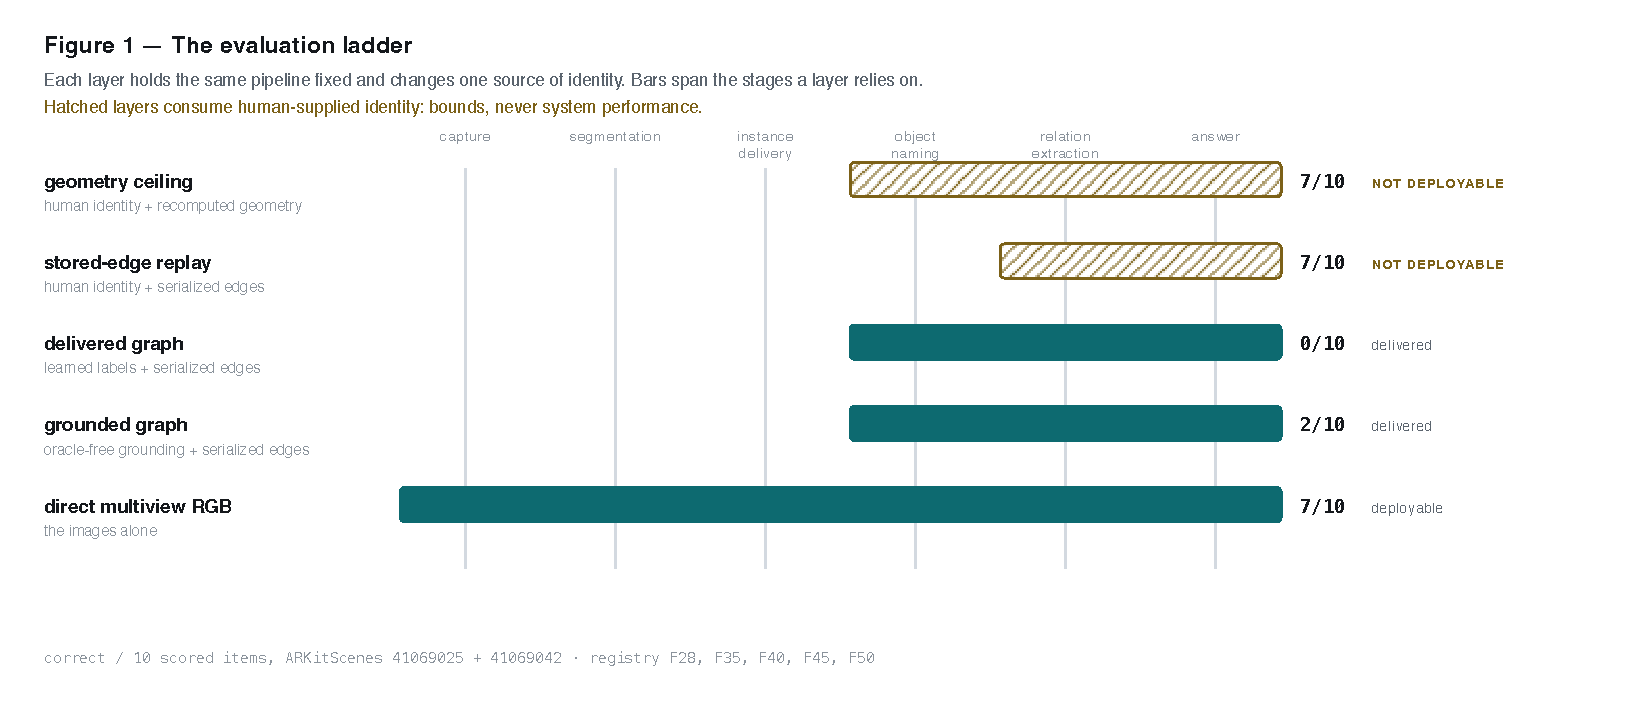
\includegraphics[width=\linewidth]{figures/fig1_evaluation_ladder.pdf}
  \caption{The evaluation ladder. Each layer holds the pipeline fixed and changes one
  source of identity; bars span the stages a layer relies on. Hatched layers consume
  human-supplied identity and are bounds, never system performance.}
  \label{fig:ladder}
\end{figure}

\subsection{Predeclaration}

Gates, stopping rules and interpretation limits are written and committed before the
corresponding scores exist. Twice this caught a \emph{structurally unreachable} outcome
before measurement: a predeclared clause that cannot fire is a broken instrument, not a
null result, and only a check in advance reveals it. In the first relation experiment the
routing structure made the accuracy clause unreachable, and it duly came in at exactly
$0.0000$ \rid{F25} with the proceed decision \texttt{false} \rid{F27}.

Blinded responses are generated in an isolated context with \textbf{no access to the key}
and hash-pinned before scoring. The protection is isolation plus the hash pin, not
version-history ordering: for the transfer run the key was recorded before the response
was pinned, so commit order does not prove the response predates the key. The full
chronology and the transfer protocol's amendment history are in the supplement.

\section{Results}

\subsection{Real capture crops as the labeler input}
\label{sec:component}

The label stage classified each delivered instance from three isolated point-splat
renders. Replacing those images with real capture RGB crops --- and changing nothing else
--- produces the largest improvement measured on any oracle-free prediction path in this
project (\cref{tab:labels}).

\begin{table}[t]
  \centering\footnotesize
  \setlength{\tabcolsep}{3pt}
  \begin{tabular}{lcccc}
    \toprule
    scene & splat t-1 & rgb t-1 & splat t-3 & rgb t-3\\
    \midrule
    A & 0/7 \rid{C05} & 5/7 \rid{C07} & 0/7 \rid{C06} & 7/7 \rid{C08}\\
    B & 1/9 \rid{C09} & 5/9 \rid{C11} & 4/9 \rid{C10} & 8/9 \rid{C12}\\
    C & 0/5 \rid{C13} & 2/5 \rid{C15} & 0/5 \rid{C14} & 3/5 \rid{C16}\\
    \midrule
    \textbf{pooled} & \textbf{1/21} \rid{C01} & \textbf{12/21} \rid{C02}
      & \textbf{4/21} \rid{C03} & \textbf{18/21} \rid{C04}\\
    \bottomrule
  \end{tabular}
  \caption{Matched-instance label accuracy. Only the images changed: weights, vocabulary,
  $\text{top\_k}=3$, admission threshold, evaluator, delivered partitions and IoU
  matching are held fixed, and no constant was tuned between scenes. The denominator is
  oracle-selected; this is not end-to-end performance.}
  \label{tab:labels}
\end{table}

\paragraph{Paired, the effect is stronger than the marginals suggest.}
Both arms were scored on the same matched instances, so the comparison is paired by
construction. At top-1, RGB fixes 12 instances and regresses 1 --- 13 discordant pairs,
exact McNemar $p = 0.0034$ \rid{G01}. At top-3 it fixes 14 and regresses none,
$p = 0.00012$ \rid{G02}. The test is the two-sided exact binomial on discordant pairs,
not the chi-square approximation, which these counts are far too small for.
\textbf{The limitation is clustering:} the 21 instances sit within only three scenes and
the test treats them as independent, which they are not --- instances in one room share a
capture, a lighting condition and a reconstruction. This is an instance-level statement,
not a scene-level or dataset-level one.

\paragraph{A control constrains the interpretation.}
A wide crop of a doorway reads as a kitchen, so a naive RGB win could have been the model
recognising \emph{rooms} rather than \emph{objects}. A third arm with wider context and
the target dimmed, run on the development scene only (7 of the 21 pooled instances),
scores \textbf{below} the tight arm at both ranks --- 3/7 \rid{C17} and 5/7 \rid{C18}
against that scene's 5/7 \rid{C07} and 7/7 \rid{C08}. More context measurably hurts,
which \textbf{supports} the interpretation that the gain comes from object texture rather
than room gist. It does not prove it.

One observation is worth recording for what it suggests rather than what it shows: six of
the 21 matched instances kept the canonical class in the top three and lost it to hard
top-1 commitment \rid{G07}. We make no claim that retaining those hypotheses would
improve question answering --- that has not been tested.

\paragraph{Scope.}
This is \texttt{oracle\_free\_component\_eval}. The prediction path consumes no oracle
and no human key, but the denominator of 21 is instances the evaluator had already
matched to an annotation box. The number is conditional on detection having succeeded and
says nothing about detection itself: on the same scenes the delivered pipeline recovered
7/18 \rid{C29}, 9/20 \rid{C30} and 5/6 \rid{C31} annotated entities. \textbf{This result
must not be reported as end-to-end or deployable performance.}

\subsection{Held but unreachable}
\label{sec:unreachable}

The central experiment asks twelve questions about \texttt{NEAR} --- the one relation the
delivered graph actually contains --- across two rooms, with ten items scored after the
owner marked two ambiguous \rid{F65}. Five layers answer the same questions over the same
stored relations, differing only in where identity comes from (\cref{tab:arms}).

\begin{table}[t]
  \centering\footnotesize
  \setlength{\tabcolsep}{3pt}
  \begin{tabular}{@{}llcc l@{}}
    \toprule
    layer & identity & correct & cov. & scope\\
    \midrule
    geometry ceiling & human & 7/10 \rid{F28} & 0.80 & \texttt{id\_oracle}\\
    stored-edge replay & human & 7/10 \rid{F35} & 0.80 & \texttt{id\_oracle}\\
    delivered graph & labels & 0/10 \rid{F40} & 0.00 & \texttt{delivered}\\
    grounded graph & bridge & 2/10 \rid{F45} & 0.20 & \texttt{delivered}\\
    direct RGB & images & 7/10 \rid{F50} & 0.90 & \texttt{deployable}\\
    \bottomrule
  \end{tabular}
  \caption{The same stored relations under five identity sources. The two 7/10 rows
  consume human-supplied identity and are bounds, not performance.}
  \label{tab:arms}
\end{table}

The direct-RGB row carries a cost the correct-count hides: on these development rooms it
was \textbf{wrong on 2 of 10} \rid{F51}. That is the baseline against which
\cref{sec:transfer}'s unseen-room behaviour must be read.

\paragraph{Relation extraction is cleared on this slice.}
The stored-edge replay reads \emph{only} edges the extractor serialized and recomputes no
geometry. It agrees with the recomputed geometry ceiling on all 12 authored items
\rid{F63}. The scope is \texttt{identity\_oracle} and the limits are real: \textbf{both
compared arms consume human-supplied identity}, the comparison covers the single
\texttt{NEAR} relation, and because both sides apply the same 1.0\,m surface-to-surface
convention the check catches a serialization error but \textbf{cannot} detect a wrong
convention.

\paragraph{Identity is what binds.}
Seven of the ten scored items are \emph{ceiling-correct, delivered-unanswered} \rid{F64}:
the delivered pipeline could not address the questions at all. Delivered-graph-unique
correct answers were 0 against a predeclared bar of 2 \rid{F60}.

\paragraph{An oracle-free bridge does not close it.}
A grounding bridge encoding anchor phrases and real capture crops with the same pinned
weights, admitting a match only on cross-view agreement and with no confidence threshold
anywhere, moved the delivered graph arm from 0/10 \rid{F40} to 2/10 \rid{F45} --- and
failed all three predeclared gates: anchor precision 0.583 against $\ge 0.80$ \rid{F67},
coverage 0.467 against $\ge 0.60$ \rid{F68}, and graph-unique wins 0 against $\ge 2$
\rid{F69}. Of the 17 question anchors, 15 were human-resolvable, the bridge admitted 12,
and 7 of those admissions were correct \rid{F70}. One failure is diagnostic: the bridge
admitted a UID for an object the owner had marked absent from the delivered partition,
with maximum cross-view agreement \rid{F75}. Cross-view agreement measures
\emph{consistency}, not \emph{existence}.

\paragraph{A ledger makes the transitions explicit.}
Rather than argue about where the capability goes, we record for each question whether it
survived each stage it must pass (\cref{fig:reach}). Of the 10 scored questions, 8 survive
object delivery \rid{G03} and all 8 survive both relation expressibility and the
serialized-edge stage --- \textbf{no question is lost to relation extraction} \rid{G05}.
Three survive anchor grounding \rid{G04}. The single largest loss, five of ten, is at
identity grounding, larger than every other transition combined. The substitution is
paired: 7 items are answered under human-supplied identity that the delivered graph does
not answer, none the other way \rid{G06}. Because one side consumes human identity, it
sizes a bound --- it says the arms differ, not that anything deployable achieves 7/10.

\begin{figure}[t]
  \centering
  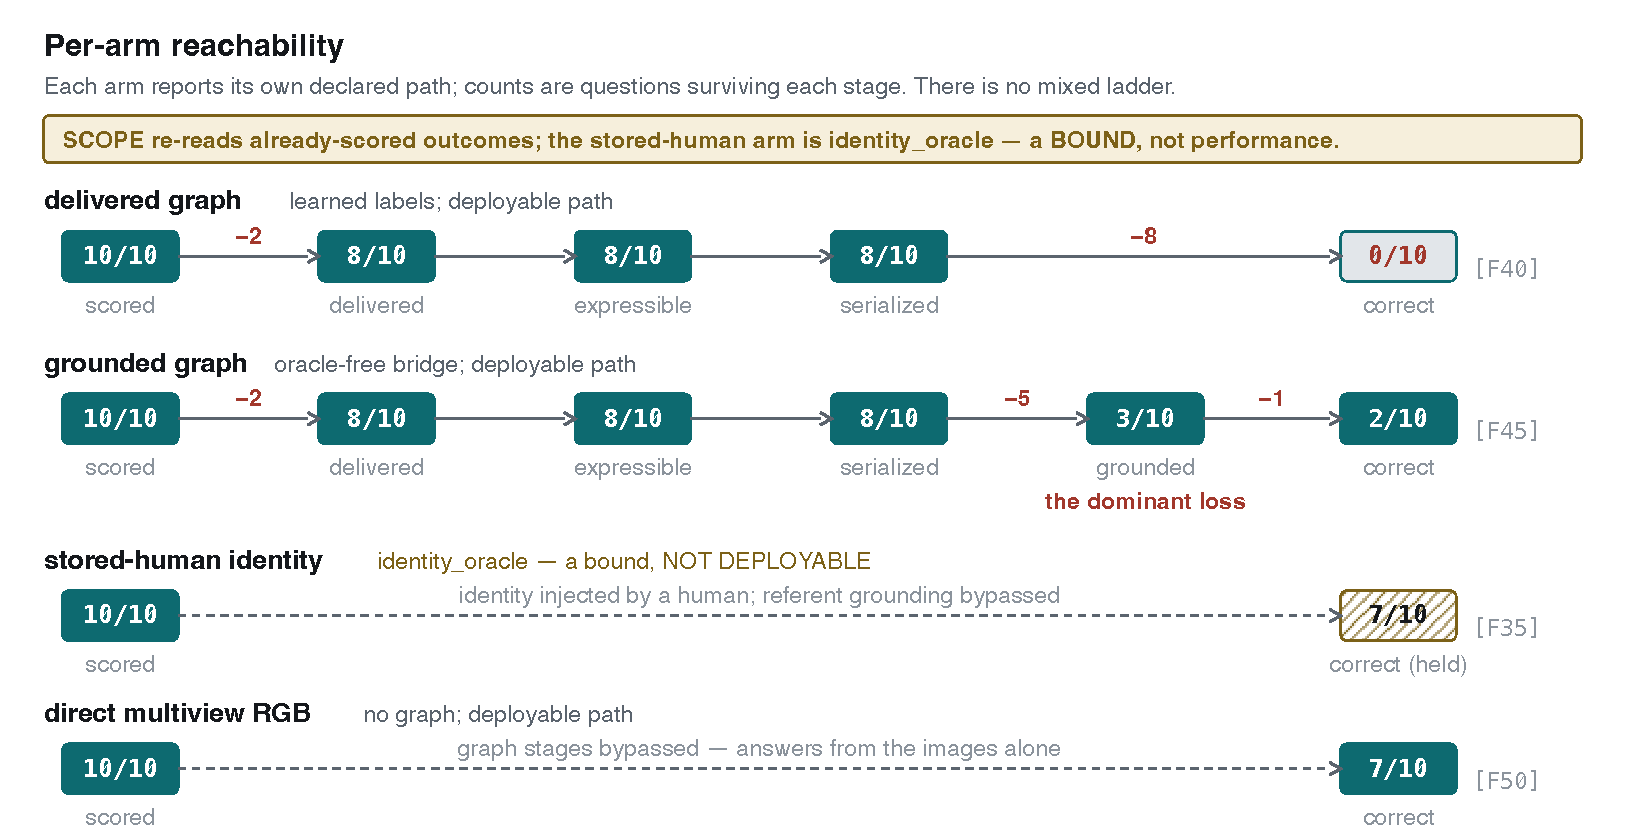
\includegraphics[width=\linewidth]{figures/fig4_reachability.pdf}
  \caption{Where questions are lost between representation and deployable answer. One row
  per stage an answer must survive. Nothing is lost at the serialized-edge stage;
  identity grounding loses more than every other transition combined.}
  \label{fig:reach}
\end{figure}

\subsection{Transfer to an untouched room}
\label{sec:transfer}

Direct multiview RGB at 7/10 \rid{F50} was the strongest deployable arm, but both rooms
had been examined for months. We froze the protocol --- question generation, view
selection, prompt, schema, scoring and two gates --- and committed it \textbf{before}
downloading a previously untouched capture. Question generation reduces direct author
selection: three agents independently enumerated objects from the same frames with no
access to each other or to any question; an object became an anchor on two-of-three
agreement; anchors were ordered mechanically and a fixed template allocated slots.

\paragraph{The generator was amended twice, and we state it plainly.}
Run 1's eight questions came back with four marked ambiguous, leaving $n = 4$ --- a size
at which the coverage gate degenerates into an anti-abstention gate. Run 1 was voided and
the generator amended twice, for scope wording and anchor ordering, then to restrict
relational slots to unique-referent anchors. What protects the result is narrower than
``we froze it first'': \textbf{the blinded model never ran in run 1}, so nothing scored
was selected on an outcome, and both amendments addressed defects visible in the
questions alone. Run 2 was authored and scored once at $n = 10$ \rid{F84}. A reader who
prefers the weaker reading --- that a generator was iterated twice on this scene before
producing a scorable set --- is entitled to it, and that is itself a finding about
fixed-procedure generation. The full amendment history is in the supplement.

\begin{table}[t]
  \centering\footnotesize
  \setlength{\tabcolsep}{3pt}
  \begin{tabular}{@{}lll@{}}
    \toprule
    metric & value & \\
    \midrule
    correct & 5/10 \rid{F76} & \\
    \textbf{wrong} & \textbf{0/10} \rid{F77} & never wrong\\
    unanswered & 5/10 \rid{F78} & \\
    acc.\ when answered & 1.000 \rid{F85} & over 5 answered\\
    \textbf{cross-view items} & \textbf{0/3} \rid{F79} & all declined\\
    exact acc.\ (gate $\ge 0.60$) & 0.50 \rid{F82} & \textbf{fail}\\
    coverage (gate $\ge 0.80$) & 0.50 \rid{F83} & \textbf{fail}\\
    \bottomrule
  \end{tabular}
  \caption{One previously untouched room, scored once. Both predeclared gates failed, so
  no transfer claim is made \rid{F88}.}
  \label{tab:transfer}
\end{table}

The shape of the failure is the result. It is not an accuracy failure: every answer given
was correct \rid{F85} and none was wrong \rid{F77}. It is entirely coverage --- and
because exact accuracy counts an abstention as a non-correct item, a perfectly calibrated
abstainer fails both gates on one behaviour. The model declined precisely the category
that motivates the work.

We resist the phrase ``calibration transferred''. On the development rooms the same arm
was \textbf{wrong on 2 of 10} \rid{F51} at 0.90 coverage \rid{F53}, and its two-view
sufficiency gate never fired on any of the 7 thin-evidence items there \rid{F66}; on the
unseen room it declined 4 of 6 thin-evidence items and was right on both it answered
\rid{F87}. That is a \emph{change} in abstention behaviour between rooms, measured once on
each, not a property carried across. This also suggests a re-reading of the earlier 7/10:
those cross-view items were likely answerable from co-visible evidence.

\section{Limitations}

\paragraph{Scale.}
Four ARKitScenes rooms (three examined during development, one first scored in the
\cref{sec:transfer} pilot) and four Replica scenes; six, twelve and ten questions per
experiment, one blinded response each, one human reviewer, who is one of the authors and is not blind to the hypothesis. The key
is itself a measurement with error: one earlier key scored a cardinality item on a
counting convention it never stated \rid{F14}, our sources still disagree on the true
count, and we report the disagreement rather than settle it. A second annotator --- blinded to
system outputs, arm names and the hypothesis --- answered all 12 items from the committed
frames: \SRAnnScoredAgree{}/\SRAnnScoredOf{} scored answers agree, every pure
disagreement is a confidence-1 abstention, and the excluded items split one--one on the
exclusion judgement \rid{G12} (details in the supplement).

\paragraph{Scope bounds.}
\Cref{sec:component}'s denominator is oracle-selected \rid{C02}, conditional on detection
succeeding and silent about detection. \Cref{sec:unreachable}'s 7/10 rows \rid{F28, F35}
consume human-supplied identity and bound what the representation could express. The
serialization check \rid{F63, G05} applies the same 1.0\,m AABB convention on both sides.
\texttt{relation\_correctness} is \texttt{unknown} on the entire ARKit slice: no
independent semantic annotation of the stored relations exists there, so serialization
consistency is the strongest relation-stage statement this paper can make.
\Cref{sec:replica}'s arms
consume oracle geometry and oracle identity, so nothing there speaks to deployable
performance; only the schema and outcome mapping transfer.
\Cref{sec:transfer} is a one-scene pilot under a twice-amended generator; both gates
failed. Every paired test in
\cref{sec:results} is instance-level; a scene-level sign test cannot reach significance
with three clusters (\cref{sec:component}).

\paragraph{An exploratory result is excluded from the claims.}
A human-keyed support experiment on one ARKit scene (1 of 3 author-confirmed positives
\rid{E27}, precision 1.0 on a single admitted candidate \rid{E28}, recall 0.3333
\rid{E29}, two of three positives on pairs captured once) is marked exploratory in the
registry and is deliberately not a headline.

\paragraph{Reproducibility.}
283 registry rows, each carrying a scope; a sanitized pack of 23 numeric reports with
checksums and provenance accompanies the paper. Twenty-eight rows
cite an untracked primary source and cannot be reproduced from the repository alone; a
further 52 quantities could not be verified against any committed artifact and are
enumerated in the census, not the registry. None is load-bearing for any claim in the
conclusion, and every registry code cited in this paper is among the verified rows of
the committed evidence pack.

\section{Conclusion}

A representation can hold information sufficient to answer questions that the deployable
query paths we instantiated do not reach: the same stored relations answer 7 of 10 with
human-supplied identity and 0 of 10 with the identity the system actually produces
\rid{F35, F40}. The measured loss on this \texttt{NEAR} slice implicates
identity access, without localizing it further: entity naming, question-to-label
matching and referent grounding are not separated for the delivered-label arm
(serialization and semantic-correctness limits: \cref{sec:limitations}).

The contributions, restated:
\begin{enumerate}\itemsep2pt \parskip0pt
  \item \textbf{The tool.} StageReach3D: per-arm paths declared as data over a fixed
  stage vocabulary, reachability derived from declared gating, reached/pass/fail/unknown
  reported separately, scope enforced in code, and outcome-keyed metrics that refuse
  pooled accuracy \rid{G09}.
  \item \textbf{The controlled validation.} \SRFaultLocalized{} artifact-level injected
  faults, spanning \SRFaultClasses{} fault classes and \SRFaultRelationTypes{} relation
  types, localized to the mutated stage while the evaluator was masked to the injected
  class, with zero false attributions on clean artifacts \rid{G11}: an
  internal-consistency check, as \cref{sec:limitations} details.
  \item \textbf{The findings.} Real RGB substantially improves the label stage on
  oracle-matched instances \rid{C01, C02, C03, C04}, a component evaluation on an
  oracle-selected denominator, \textbf{not end-to-end or deployable performance}, with
  a control supporting but not proving the object-texture reading \rid{C17, C18}.
  Stored relations hold answers under human-resolved identity that deployable grounding
  does not reach \rid{F35, F40, F45}. Direct RGB is the strongest measured path on the
  two development rooms \rid{F50, F53}, though wrong on 2 of 10 there \rid{F51},
  under one named model (claude-opus-5), one frozen pass; on the pilot room it answered
  5 of 10 with zero wrong answers \rid{F76, F77} and failed both predeclared gates
  \rid{F82, F83}, so no cross-room claim is made. Every number is
  instance-bound; what is designed to transfer is the evaluator.\label{endofmaintext}
\end{enumerate}


{
    \small
    \bibliographystyle{ieeenat_fullname}
    \bibliography{refs}
}

\end{document}
